\begin{center}
\footnotesize Originale verkita de J. \fsc{Grohn}, privata instruisto.
\end{center}

   Rigardu tiun \^ci figuron, kiu prezentas la montran fingron de la
maldekstra mano,

\begin{center}
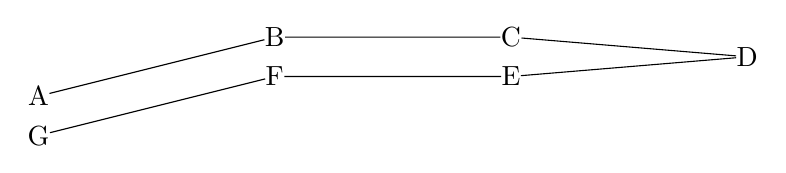
\begin{tikzpicture}[every node/.style={inner sep=0pt}]
\node[align=center](A) at (0,0.5){A} ;
\node[align=center](B) at (3,1.25){B} ;
\node[align=center](C) at (6,1.25){C} ;
\node[align=center](D) at (9,1){D} ;
\node[align=center](E) at (6,0.75){E} ;
\node[align=center](F) at (3,0.75){F} ;
\node[align=center](G) at (0,0){G} ;
\draw(A) -- (B) -- (C) -- (D) -- (E) -- (F) -- (G);
\end{tikzpicture}
\end{center}

%         (la literoj estas konektitaj per strekoj la\u ualfabete)
%
%                                    B          C
%   fingro-pintoj:         A                               D
%                                    F          E
%   fingro-artikoj:        G

   sur kiu la lokoj de fleksoj kaj la fineto de la fingro estas signitaj
per sep literoj A, B, C, D, E, F, G. Tiuj \^ci sep punktoj prezentas
la sep tagojn de semajno. \^Ciu devas sur sia propra fingro signi
tiujn \^ci punktojn en penso per tiuj \^ci sep literoj kaj en tiu
sama ordo, kiel ni vidas sur la figuro.

   Anta\u u ol ni iros pli malproksimen, ni devas bone lerni parkere
la sekvantan frazon sisteman, sen kiu oni ne povas uzi nian fingran
kalendaron:

\begin{quote}
{\bf A}lta {\bf D}ia {\bf d}ono,\\
{\bf G}randa {\bf b}en', {\bf e}spero!\\
{\bf G}vidu {\bf \^c}ion {\bf f}irme\\
{\bf A}l {\bf d}ezira {\bf f}ino.
\end{quote}

   Tiu \^ci frazo estas kunmetita el dekdu vortoj, kies unuaj literoj
montras al ni, de kiu punkto sur la fingro \^ciu monato komencas
kalkuli siajn tagojn.

   Jen estas la sistemo monata:

\begin{table}[h]
\centering
\begin{tabu} to\textwidth{@{}c@{ }c@{ }l@{ }c@{ }l}
 $1^{\small{a}}$  & monato & (Januaro)    & komencas de la punkto & A (alta)\\
 $2^{\small{a}}$  &   --   & (Februaro)   &          --           & D (dia)\\
 $3^{\small{a}}$  &   --   & (Marto)      &          --           & D (dono)\\
 $4^{\small{a}}$  &   --   & (Aprilo)     &          --           & G (granda)\\
 $5^{\small{a}}$  &   --   & (Majo)       &          --           & B (ben')\\
 $6^{\small{a}}$  &   --   & (Junio)      &          --           & E (espero)\\
 $7^{\small{a}}$  &   --   & (Julio)      &          --           & G (gvidu)\\
 $8^{\small{a}}$  &   --   & (A\u ugusto) &          --           & C (\^cion)\\
 $9^{\small{a}}$  &   --   & (Septembro)  &          --           & F (firme)\\
 $10^{\small{a}}$ &   --   & (Oktobro)    &          --           & A (al)\\
 $11^{\small{a}}$ &   --   & (Novembro)   &          --           & D (dezira)\\
 $12^{\small{a}}$ &   --   & (Decembro)   &          --           & F (fino).\\
\end{tabu}
\end{table}

   Se vi volas scii, kial la sistemo monata devas esti difinita tiel
kaj ne alie, kalkulu sur la punktoj de la fingro kaj vi vidos, ke se
la monato Januaro, havanta 31 tagojn, komenci\^gas de la punkto A
(Alta), \^gi fini\^gas sur la punkto C; la dua monato, Februaro,
havanta 28 tagojn (en jaro simpla) komenci\^gas de la punkto D
(\^car la 31\textsuperscript{a} de Januaro estis c) kaj fini\^gas sur C; la tria
monato, Marto, komencas kalkuli siajn tagojn de la punkto D, k. c.
(Pri superjaro, t. e. jaro 366-taga ni parolos poste.)

{\it Rimarko.} \^Ce kalkulado \^cirka\u u la fingro oni povas facile
vidi, ke la datoj 8, 15, 22 kaj 29 de \^ciu monato \^ciam falas sur
tiun saman punkton, de kiu la monato komenci\^gas.

{\sl Ekzemplo 1.} De kiu punkto komenci\^gas Aprilo?
--- {\sl Solvo:} Aprilo, la kvara monato, komenci\^gas de la punkto, kiu estas
signata per la unua litero de la kvara vorto de la frazo (G).

{\sl Ekzemplo 2.} Sur kiu punkto sin trovas la 5 de Novembro?
 --- {\sl Solvo:} Al Novembro, la dekunua monato, respondas la dekunua vorto
de la frazo (Dezira) kaj tiel la punkto D estas la unua, E la dua, F
la tria, G la kvara kaj A estas la kvina tago de Novembro.

{\sl Ekzemplo 3.} Sur kiu punkto sin trovas la 23 de Junio?
--- {\sl Solvo:} Al Junio, la sesa monato, respondas la sesa vorto de la
frazo (Espero) kaj tiel la punkto E estas la 1, 8, 15 kaj 22 kaj F
estas la 23 tago de la monato Junio.

   Nun ni vidos, kiun nomon de tago semajna \^ciu punkto de la fingro
devas havi:

{\sl Ekzemplo 4.} Ni elser\^cu la punkton de la hodia\u ua tago,
supozante, ke hodia\u u estas \^{\j}a\u udo la 8 de Majo de la jaro
1890. ({\it Rimarko.} Kiu lernas tiun \^ci kalendaron, ne devas sin
teni je nia supozita tago, nombro kaj monato, \^car estos pli klare
kaj pli kompreneble, se li prenos por ekzemplo la daton kaj la nomon
de tiu tago, en kiu li lernas, kaj solvos sian ekzemplon konforme je
la sekvanta solvo).
--- {\sl Solvo:} Al Majo, la kvina monato, respondas
la kvina vorto de la frazo (Ben'), kaj tiel la punkto B estas la 1
kaj la 8 de Majo; kaj \^car ni scias, ke tiu \^ci tago estas
\^{\j}a\u udo, ni facile konkludas, ke la punkto B estas \^{\j}a\u
udo, C --- vendredo, D --- sabato, E --- diman\^co, F --- lundo, G
--- mardo kaj A --- merkredo. Tiuj \^ci nomoj de tagoj restas por la
punktoj por tiu \^ci tuta jaro 1890.

{\it Rimarko.} Por ne \^sar\^gi la memoron, estas sufi\^ce nur
memori la punkton de diman\^co, kaj el la anta\u uiranta solvo ni
vidas, ke por tiu \^ci jaro (1890) la punkto E estas la diman\^co.

   En la sekvanta jaro la nomoj de la tagoj transiras sur la
anta\u uirantajn punktojn, kaj \^gi fari\^gas pro jena ka\u uzo: se
la simpla jaro havus nur precize 52 semajnojn, \^gi komenci\^gus de
la punkto A (en nia jaro --- merkredo) kaj fini\^gus sur la punkto G
(mardo), kaj la estonta jaro komenci\^gus ree de A kaj la tagoj por
la punktoj restus tiuj samaj sen \^san\^go; sed beda\u urinde la
jaro ekster 52 plenaj semajnoj havas ankora\u u unu superfluan
tagon, sekve \^gi ne povas fini\^gi sur la punkto G (mardo), sed
\^gia fino estos A (merkredo) kaj la estonta jaro devas komenci\^gi
de la sekvanta tago (\^{\j}a\u udo), sed ne de la sekvanta punkto B,
\^car la sistemo monata postulas por la monato Januaro la punkton A
(Alta). Por konsentigi tiujn \^ci du postulojn (ke la estonta jaro
komenci\^gu de la punkto A kaj de \^{\j}a\u udo), oni devas diri, ke
kun la komenco de nova jaro la ordo de la nomoj de tagoj por la
punktoj de la fingro \^cesi\^gas kaj komenci\^gas nova ordo, tio
estas: la punkto A akceptas la nomon de la tago, kiun la punkto B
\^gis tiu tempo havis. Sekve, vidante ke en tiu \^ci jaro 1890 B
estas \^{\j}a\u udo, ni scias, ke kun la komenco de la estonta jaro
A estos \^{\j}a\u udo kaj la punkto diman\^ca anstata\u u E en la
estonta jaro estos D.

   Nun estas anka\u u facile kompreni, ke por la 29\textsuperscript{a} tago de Februaro
en superjaro devas veni tia sama \^san\^go de la nomoj de tagoj por
la punktoj de la fingro. Nia sistemo kalendara estas verkita por
jaro simpla, en kiu la monato Februaro havas nur 28 tagojn kaj tiel,
komenci\^gante sur la punkto D, tiu \^ci monato fini\^gas sur C kaj
la sekvanta monato Marto komenci\^gas de la punkto D. Sed \^car en
superjaro Februaro havas ankora\u u unu tagon, sekve \^gi ne povas
fini\^gi sur C, sed devas fini\^gi sur D kaj la sekvanta monato
devas komenci\^gi de la sekvanta tago, sed ne de la sekvanta punkto
E, \^car la sistemo monata postulas por la monato Marto la punkton
D. Sekve ni vidas, ke por konsentigi tiujn \^ci 2 postulojn (ke la
monato Marto komenci\^gu de la punkto D kaj de la sekvanta tago), ni
devas diri, ke en la komenco de Marto la anta\u ua ordo de la nomoj
de tagoj por la punktoj sur la fingro \^cesi\^gas kaj en la komenco
de Marto en superjaro la punkto D akceptas la nomon de la tago, kiun
la punkto E \^gis tiu tempo havis. Sekve, transirante de jaro simpla
en sekvantan superjaron, ni havas 2 \^san\^gojn de la nomoj de tagoj
por la punktoj: unu fojon por Januaro kaj Februaro kaj la duan fojon
por la lastaj 10 monatoj. Tiel en tiu \^ci jaro 1890 la diman\^co
estas sur la punkto E, en la estonta jaro 1891 \^gi estos sur D kaj
en la superjaro 1892 la diman\^co estos sur C por la unuaj du
monatoj kaj sur B por la lastaj dek; tio estas: la nomoj de tagoj
sin \^sovas posten en returnita ordo de la alfabeto.

{\it Rimarko.} El tiu \^ci klarigo estas facile kompreni, ke se oni
volas ser\^ci ian tagon en pasinta tempo, oni devas \^sovi la nomojn
de tagoj por \^ciu jaro en rekta alfabeta ordo: tio estas, se en tiu
\^ci jaro 1890 la punkto diman\^ca estas E, sekve en la pasinta jaro
1889 \^gi estis F kaj en 1888 (superjaro) la punkto diman\^ca estis
G por la lastaj dek monatoj kaj A por la unuaj du monatoj k. c.

   \^Ciuj \^gis nun donitaj reguloj montras al ni, kiel trovi la tagon,
se oni scias la nombron en la monato (la daton); nun kiel oni trovos
la daton, se oni scias la tagon? Ekzemple: hodia\u u estas vendredo
en Oktobro, --- kian daton ni donos al tiu \^ci vendredo, sciante,
ke \^ciu tago ripeti\^gas kvar a\u u kvin fojojn en la monato?

   Tiel sciu: se iu en la da\u uro de longa tempo ne rigardis la daton,
tiu anka\u u el presita kalendaro ne scios la daton por la demandata
tago, \^car la kalendaro al ni ne povas diri, kiu vendredo en
Oktobro \^gi estas; sed se li memoras, ke en unu el la lastaj tagoj
ni havis ekzemple la na\u uan de Oktobro, tiam al li estos facile
reser\^ci tiun \^ci daton sur la fingro kaj poste trovi la plej
proksiman vendredon. En tia okazo ni divas: Oktobro, la deka monato,
komenci\^gas sur la punkto, kiu estas signata per la unua litero de
la deka vorto de nia frazo (Al), t. e.: A estas la 1 kaj 8, B --- la
9 de Oktobro; kaj \^car E en tiu \^ci jaro 1890 estas diman\^co,
tial B a\u u la 9 de Oktobro estos \^{\j}a\u udo kaj la sekvanta
vendredo estos la 10.

   Okazas iafoje, ke oni volas difini la tagon por ia dato en
malproksima jaro, por kiu difini la punkton de diman\^co estas ne
facile kaj e\^c lacige. En tia okazo (konsiderante, ke \^ciu simpla
jaro havas unu superfluan tagon super la nombro de semajnoj kaj la
superjaro havas ilin du) ni devas la nombron de \^ciuj tiuj \^ci
superfluaj tagoj, kiuj sin trovas en la intertempo inter la kuranta
jaro kaj la ser\^cata, dividi je sep, t. e. tiujn \^ci tagojn turni
en x semajnojn, kaj la resto al ni montros, je kiom punktoj ni devas
\^sovi la punkton diman\^can (la\u u ordo alfabeta). Se la divido
fari\^gis sen resto, tiam la punkto diman\^ca en la ser\^cata jaro
estas tiu sama, kiel en ia kuranta jaro.

{\it Rimarko 1\textsuperscript{a}.} Rilate la lastan regulon por difini la tagon en
malproksima jaro (\^ce kiu ni diris, ke ni devas dividi je sep la
nombron de la superfluaj tagoj, kiuj sin trovas en la intertempo
inter la kuranta jaro kaj la ser\^cata) ni devas fari la rimarkon,
ke se ni trovi\^gas en la lastaj dek monatoj de superjaro, ni devas,
\^ce la elkalkulado de la superfluaj tagoj, aldoni ankora\u u unu
tagon por la 29\textsuperscript{a} Februaro de la kuranta jaro. Tiel same oni devas
agi, se la ser\^cata dato trovi\^gas en Januaro a\u u Februaro de ia
superjaro.

{\it Rimarko 2\textsuperscript{a}.} Ser\^cante ian daton en pasintaj centjaroj, ni
devas meti atenton sur la lastan jaron de la centjaro, kiu, malgra\u
u ke la nombro de la jaro estas dividebla je 4, nur tiam estas
superjaro, kiam la nombro de la centjaro dividas sin je 4. Sekve la
jarojn 1700, 1800 kaj 1900 ni devas kalkuli al la jaroj simplaj kaj
ne al superjaroj, \^car la nombro 17, 18 kaj 19 ne estas divideblaj
je 4.

   \^Ciuj reguloj de nia fingra kalendaro povas esti uzataj tiel same por
la Julia kalendaro (malnova stilo), nur kun tiu diferenco, ke la
punkto de diman\^co falas \^ciam sur la duan sekvantan punkton post
tiu, kiu en la kalendaro Gregoria (nova stilo) signifas la
diman\^con; se tiel la\u u la kalendaro Gregoria D signifas la
diman\^con por la kuranta jaro 1891, la diman\^co la\u u la malnova
stilo estos sur la punkto F. Sed ni devas sciigi niajn karajn
legantojn, ke la lasta rimarko (pri la lastaj jaroj de centjaroj)
tie \^ci ne povas havi lokon.

   Nun, estimataj amikoj de nia lingvo, se vi komprenas \^ciujn regulojn
de nia kalendaro, tiam ne estos al vi malfacile solvi la sekvantajn
du temojn:

   1\textsuperscript{a} Difinu la tagon de la morto de Koperniko, kiu mortis la 12\textsuperscript{an} de
Februaro de la jaro 1473.

   2\textsuperscript{a} Trovu, en kiu tago naski\^gis Kristo?

{\it Rimarko.} \^Ce la amba\u u temoj devas esti uzata la kalendaro
Julia, \^car la Gregoria komenci\^gis de la jaro 1583.

\smallrule{}
